% Sistema térmico: cuerpo con capacitancia C y resistencia R al ambiente
\documentclass[border=5pt]{standalone}
\usepackage{tikz}
\usetikzlibrary{arrows.meta}
\begin{document}
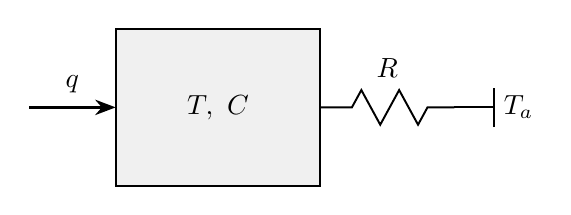
\begin{tikzpicture}[>={Stealth[length=2.6mm]}, line width=0.7pt]
  % cuerpo (capacitancia termica)
  \draw[fill=black!6] (0,0) rectangle (2.6,2.0);
  \node at (1.3,1.0) {$T,\ C$};
  % flujo de calor de entrada
  \draw[->, line width=1pt] (-1.1,1.0) -- (0,1.0);
  \node[above] at (-0.55,1.05) {$q$};
  % resistencia termica al ambiente (zigzag)
  \draw (2.6,1.0) -- (3.0,1.0)
        -- ++(0.12,0.22) -- ++(0.24,-0.44) -- ++(0.24,0.44) -- ++(0.24,-0.44) -- ++(0.12,0.22)
        -- (4.3,1.0);
  \node[above] at (3.45,1.25) {$R$};
  % ambiente
  \draw (4.3,1.0) -- (4.8,1.0);
  \node[right] at (4.8,1.0) {$T_a$};
  \draw (4.8,0.75) -- (4.8,1.25);
\end{tikzpicture}
\end{document}
